\documentclass{article}

% Language setting
% Replace `english' with e.g. `spanish' to change the document language
\usepackage[english, russian]{babel}
\usepackage{amsmath}


\usepackage{wrapfig}
\usepackage{graphicx}
\usepackage{pgfplots}


%%% Работа с картинками
\usepackage{graphicx}  % Для вставки рисунков
\graphicspath{{images/}{images2/}}  % папки с картинками
\setlength\fboxsep{3pt} % Отступ рамки \fbox{} от рисунка
\setlength\fboxrule{1pt} % Толщина линий рамки \fbox{}
\usepackage{wrapfig} % Обтекание рисунков и таблиц текстом

 % для диаграмм
\usepackage{pgf}
\usepackage{tikz}
\usepackage[utf8]{inputenc}
\usetikzlibrary{arrows,automata}
\usetikzlibrary{positioning}
\tikzset{
    state/.style = {draw, rounded corners, 
                 minimum width=22mm, minimum height=5mm, align=center},
}


\usepackage{tcolorbox}

% Set page size and margins
% Replace `letterpaper' with `a4paper' for UK/EU standard size
\usepackage[letterpaper,top=2cm,bottom=2cm,left=3cm,right=3cm,marginparwidth=1.75cm]{geometry}

% Useful packages
\usepackage{amsmath}
\usepackage{amssymb}
\usepackage{graphicx}
\usepackage{fixltx2e}
\usepackage[colorlinks=true, allcolors=blue]{hyperref}
\usepackage{pgf}
\usepackage{array}
\newenvironment{conditions}
  {\par\vspace{\abovedisplayskip}\noindent\begin{tabular}{>{$}l<{$} @{${}={}$} l}}
  {\end{tabular}\par\vspace{\belowdisplayskip}}

\usepackage{geometry}
\geometry{left=25mm,right=25mm,
 top=25mm,bottom=25mm}

\title{Quantitative Analytics.\\
Lectures. Week 5-8. \\
UNDERSTANDING THE BALANCE SHEET}
\author{Дмитрий Базанов}

% Колонтитулы
\usepackage{fancyhdr}
\pagestyle{fancy}
\renewcommand{\headrulewidth}{0.1mm}  
\renewcommand{\footrulewidth}{0.1mm}
\lfoot{}
\rfoot{\thepage}
\cfoot{}
\rhead{CMF-2022}
\chead{}

\begin{document}
\maketitle

% Оглавление
\setcounter{tocdepth}{1} % {2} - в оглавлении участвуют chapter, section и subsection. {1} - только chapter и section
\renewcommand\contentsname{Contents}
\tableofcontents
\newpage



\renewcommand{\labelitemi}{\tiny$\bullet$}
\renewcommand{\figurename}{Fig.}


\section{Что такое балансовый отчёт?}
	Есть тесная связь между балансовым отчётом и отчётом о прибылях и убытках. В отчёте о прибылях и убытках в основном отражены переменные потока, баланс же состаявляет своего рода "фотографию" компании в определённый момент времени в переменных состояния. 
   
\section{ Из чего состоит балансовый отчет? }
\begin{enumerate}
\item \textbf{Активы(assets)} -- источник будущих возможных экономических выгод, которые могут быть получены компанией как результат предыдущих транзакций. Могут быть получены в следствие: обычных операция компании, инвестиционные действия, финансовая активность. К активам отновится всё то, отчего "нам хорошо".

\item \textbf{Пассивы(liabilities)} -- обязательства. То, что мы должны сделать в силу предыдущих действий, транзакций, ведут к оттоку экономических выгод: счета к оплате, накопленные расходы, векселя, облигации к погашению, лизинг, отложенные налоги, пенсионные обязателсьтва перед работниками. 

\item \textbf{Собственный капитал(equity)} -- это остаточный компонент в активах, в который входит всё, что остается после исполнения всех обязательств. Это собственность акционеров, они получают прибыль в последнюю очередь, рискуют больше всех.

Чаще всего собственный капитал возникает при активностей по привлечению финансирования – например, выпуск акций, иногда операционные действия. 
В собственный капитал входят:
\end{enumerate}
    
\begin{itemize}
\item \textbf{Capital stock} – то, что было вложено изначально.
\item  \textbf{Addidtional paid-in-capital}–  то, что добавили, если продали, например, акции дороже.
\item \textbf{Treasury stock shares }– это те акции, которые можно было бы продать и распределить между акционерами.
\item \textbf{Accumulated retained earnings} –   Накопленная нарастающим итогом нераспределенная прибыль.
\item  \textbf{Accumulated other comprehensive income} – накопленный нарастающим итогом прочий доход.
\end{itemize}
                        
			 \section{ Использование balance sheet в финансовом анализе}

Самое главная сложность в использовании балансового отчета – это то, что данные в нем могут сильно расходиться с реальной картиной мира. Если здания и сооружения значатся на балансе по некой цене, это не означает, что они могут быть проданы за эту сумму.

Например, встречаются ситуации, когда хорошо функционирующие производственные комплексы являются имуществом с нулевой балансовой стоимостью, потому что они достаточно старые. Бывают и обратные случаи. 

\textbf{Почему так происходит?}

Какие-то элементы баланса отражаются по исторической стоимости, не амортизируясь. Некоторые компоненты баланса амортизируются – каждый период частично списывается порция стоимости. Некоторые могут отражаться по рыночной стоимости, если она известна. 

Некоторые компоненты в принципе нельзя отразить в балансе: репутация, требования как к эмитентам облигаций, судебные разбирательства.
Тем не менее, баланс может рассказать о ликвидности (возможность исполнять краткосрочные финансовые обязательства) , платежеспособности (возможность исполнять долгосрочные финансовые обязательства), возможно делать выплаты акционерам.

\section{В какой форме может быть предоставлен балансовый отчет?}
Жёсткого стандарта нет. Однако можно выделить два основных подхода:
\textbf{Баланс с разбивкой по счетам }– формат, в котором справа находятся пассивы и собственный капитал, слева - активы. 
\textbf{Другой формат} – активы, пассивы и капитал в одной колонке. 

Еще одна важная особенность формата баланса – он традиционно классифицирован. Вместе группируются схожие единицы, обязательна категоризация по текущим и не текущим (долгосрочным) пассивам и активам, то есть по ликвидности.

\section{Оборотные (текущие) активы}

\textbf{Оборотные активы (current assets) }– денежные средства и другие активы, которые могут быть конвертированы в денежные средства или использованы в течение одного года или операционного цикла после даты, на которую предоставляется отчёт.

\textbf{Операционный цикл }– период, в течение которого фирма закупает или производит продукт (формирует запас на складе), реализует его и получает за это деньги. 

Текущие активы презентуются в порядке их ликвидности, начиная с денежных средств и их эквивалентов:

\begin{itemize}
\item \textbf{Cash and cash equivalents }– ликвидные низко рискованные ценные бумаги со сроком погашения меньше 90 дней. Измеряются по рыночной или амортизационной стоимости, если они постепенно растут к погашению.
\item \textbf{Accounts receivable }– сумма, которую мы ожидаем получить за проданные товары или предоставленные услуги за вычетом сомнительных платежей и скидок 
\item \textbf{Inventories} – то, что мы храним на складе, чтобы продать или использовать в производстве: сырье, материалы, незавершенное производство, законченные товары. Для оценки используются самые низкие оценки - по себестоимости (стоимость покупки, транспортировки и обработки) - или по чистой продажной стоимости. Есть несколько способов отражать их в балансе: LIFO (не используется в МСФО), FIFO, AVG.
\item \textbf{Marketabke securities} – долевые и долговые ценные бумаги, которые торгуются на организованных рынках, отражаются по рыночной справедливой стоимости (AFS – available for sale) или по амортизационной стоимости (HTM -  hold to maturity).
\item \textbf{Prepaid expenses} – аванс, оплаченный за предоставление товаров или услуг в будущем.
\item \textbf{Deferred tax assets} – налоги, не отраженные в Pnl, появляются в случае, если компания заплатила слишком много и получит налоговое освобождение или налоговый возврат (только в США по GAAP, в МСФО все возможные налоговые активы отражаются как не текущие).
\item \textbf{Other current accounts }– все, что не вошло в вышеперечисленные разделы.
\end{itemize}



\section{Необоротные (не текущие) активы}

\textbf{Необоротные активы(non-current assets )} – активы, которые не будут конвертированы в денежные средства или полностью использоваться в течение одного года или операционного цикла. В них входит капитальная база, которую фирма использует для производства: здания, сооружения, патенты, лицензии, права.
\begin{itemize}
\item \textbf{Property plant and equipment }– материальные  активы, которые используются в производстве – земля, здания, сооружения. Могут отражаться следующими способами: 
\begin{itemize}
\item \textbf{Cost model} –  используется историческая стоимость за вычетом  накопленного объема обесценения (износ, падение рыночных цен, порча) – требуется регулярно проверять на резкое снижение стоимости данной строки активов. В GAAP отражаются только таким методом.
\item \textbf{Revaluation model} – используется справедливая стоимость за вычетом обесценения. Только в МСФО.
\end{itemize}

\item \textbf{Investment property} – материальные активы, которые позволяют получать рентный доход или имеют потенциал для изменения стоимости. Отражаются по справедливой или остаточной (амортизационной) стоимости.
\item \textbf{Intangible assets }– неденежные активы (не ценные бумаги), у которых нет физического проявления.
\begin{itemize}
\item \textbf{Identifiable} -- патенты, права на использования, торговые марки. Отражаются по себестоимости или периодически переоцениваются, стоимость списываетсяна протяжении срока использования.
\item \textbf{Unidentifiable } – goodwill - создается при покупке чего-либо, когда покупатель заплатил сумму, превышающую стоимость активов, "заплатка" в балансе. Нет амортизации, но регулярно проверяется на возможность списания.
\end{itemize}
Нематериальные активы, которые созданы засчёт внутренних резервов (R&D), по GAAP отражаются как расходы, по МСФО можно списывать расходы постадийно, но когда начинается создание годного образца, можно записать как актив в балансе. Затраты, которые должны быть списаны в PnL во всех стандартах:
				
\begin{itemize}
\item Затраты на прекращение исследований.
\item Рекламные и промоутинговые расходы (на продвижение, рекламу, маркетинговые исследования).
\item Себестоимость запуска и обучения работников.
\item Стоимость перемещения и реорганизации рабочей силы.
\end{itemize}
\end{itemize}

\section{Оборотные (текущие) обязательства}
\textbf{Текущие обязательства} – обязательства, которые должны быть выполнены в течение одного года или одного операционного цикла. Чтобы обязательства были признаны текущими, ожидается, что мы их исполним в течение этого периода.  

\begin{itemize}
\item \textbf{Accounts payables} – неоплаченные счета, выставленные поставщиками товаров и услуг.
\item \textbf{Notes payable and current portion of long-term debt} - то, что мы должны заплатить по векселям и по текущей порции долгосрочных долгов. 
\item \textbf{Accured expenses} – расходы, признанные начисленными, но еще не оплаченные (проценты, платежи аренды, которые обычно платятся в конце месяца или года).
\item \textbf{Unearned revenue} – то, что получили авансом за товары или услуги.
\end{itemize}



\section{Необоротные (не текущие) обязательства}
\begin{itemize}
\item \textbf{Long term financial liability} – банковские займы, векселя, облигации к погашению, производные финансовые инструменты. Отражаются по амортизационной стоимости (для займов) или по справедливой рыночной стоимости (для производных финансовых инструментов, деривативов).
\item \textbf{Deferred tax liability} – возникают, когда уплечаено налогов меньше, чем нужно, и мы ожидаем, что налоговая инспекция может потребовать доплатить большую сумму. В основном учитываются в GAAP, по МСФО все отложенные налоги не текущие.
\begin{itemize}
\item Классифицируются согласно тому, на что накладывается налог берется (какие сроки у активов, связанных с налогом).
\item Ожидаемое время восстановления платежа или выплаты с нашей стороны.
\end{itemize}

\end{itemize}

\section{Компоненты акционерного капитала }
\textbf{Shareholders equity} – то остаточный компонент в активах, в который входит всё, что остается после исполнения всех обязательств. 
\begin{itemize}
\item \textbf{Owners equity} -то, что осталось.
\item \textbf{Capital stock (contributed capital issued capital) }– то, что изначально вложили
\item \textbf{Additional paid-in-capital} – добавочный капитал\textit{ in excess of par }, который появляется при продаже акций по цене выше номинальной.
\item \textbf{Treasury stock} – те акции, кот можем выпустить и продать (значатся на балансе по некоторой прогнозной стоимости), превратив в \textit{issued shares} – акции, которые можем поглощать обратно  (показатель, который просто значится на балансе).
\item \textbf{Autorise shares} – то количество акций, которое мы имеем право выпустить согласно уставным документам.
\item \textbf{Retained earnings } (нераспределенная прибыль) – прибыль, не выплаченная в виде дивидендов акционерам и реинвестированная в бизнес, накапливается за время жизни компании.
\item \textbf{Accumulated other comprehensive income} – другой доход, который накапливается постепенно.
\item \textbf{Сontributed capital } - общее количество капитала, которое привнесено владельцами обычных и привилегированных акций.
\item  \textbf{Par value} – номинальная стоимость акций.
\end{itemize}

\section{Как использовать баланс в сравнительном анализе?}
Конвертация обычного баланса в приведенный вид (каждый счёт как процент общих активов ,vertical common sixe analysis) позволяет, во-первых, посмотреть на отношение компонентов баланса относительно друг друга, во-вторых. на изменение баланса фирмы по отношению к другим фирмам (конкурентам), в-третьих, сравнить со среднеиндустриальными показателям.

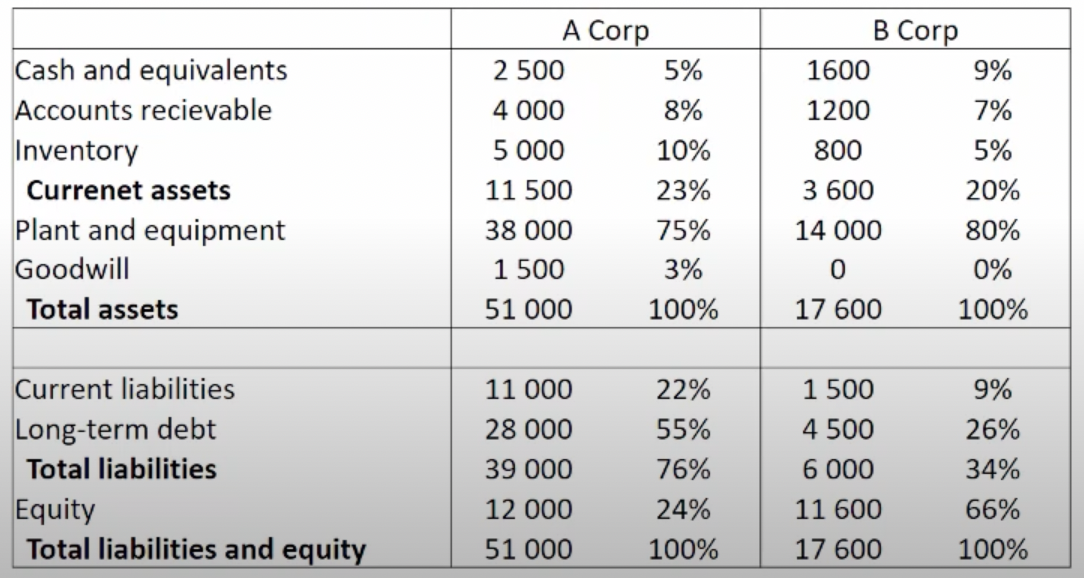
\includegraphics[width=150mm]{common-size.png}


\section{Балансовые коэффициенты}
Помимо соотнесения всех компонент баланса с активами, можно посчитать еще \textit{liquidity ratios}, \textit{solvency rations}. Это исключительно балансовые коэффициенты, поскольку все компоненты для расчета считываются с баланса.

\textbf{Коэффициенты ликвидности(liquidity ratios)} показывают возможности компании по выполнению краткосрочных обязательств.

\textbf{Коэффициенты платёжеспособности (solvency ratios)} показывают возможности выполнения долгосрочных обязательств.

Общий принцип – чем выше коэффициент, тем более вероятно выполнение обязательства.

\textbf{{Liquidity ratios}}

$$\text{current ratio} = \frac{\text{current assets}}{\text{current liabilities}}$$

$$\text{quick ratio} = \frac{\text{cash+marketable securities + receivables}}{\text{current liabilities}}$$

$$\text{cash ratio} = \frac{\text{cash+marketable securities}}{\text{current liabilities}}$$

\textbf{Solvency ratios}:
Здесь наоборот, чем больше коэффициент, тем больше вероятность неисполнения обязательств.

$$\text{long-term debt to equity ratio} = \frac{\text{total long term debt}}{\text{total equity}}$$

$$\text{debt to equity ratio} = \frac{\text{total debt}}{\text{total equity}}$$

$$\text{total debt to equity ratio} = \frac{\text{total debt}}{\text{total assets}}$$

$$\text{financial leverage} = \frac{\text{total assets}}{\text{total equity}}$$


Эти коэффициенты нужно сопоставлять с компаниями, занятыми схожими видами бизнеса, но относиться с осторожностью (разница в принципах расчета, стандартах учета).



 \end{document}
 
  